\documentclass[11pt,a4paper,UTF8,fontset=fandol]{ctexart}

\usepackage[a4paper,margin=2.45cm,headheight=14pt]{geometry}
\usepackage{booktabs}
\usepackage{tabularx}
\usepackage{array}
\usepackage{longtable}
\usepackage{float}
\usepackage{enumitem}
\usepackage{setspace}
\usepackage{fancyhdr}
\usepackage[hidelinks]{hyperref}
\usepackage{microtype}
\usepackage{graphicx}
\usepackage{xcolor}
\usepackage{tikz}
\usetikzlibrary{arrows.meta,positioning,calc}

\hypersetup{
  pdftitle={Voice-Driven PowerPoint Editing Agent: SURF Project Experimental Report},
  pdfauthor={},
  pdfsubject={From PPTArena Reproduction to ASR-Agent Experiments},
  pdfkeywords={SURF, PowerPoint, PPTArena, PPTPilot, ASR, Agent}
}

\setstretch{1.25}
\setlength{\parindent}{2em}
\setlength{\parskip}{0pt}
\setlength{\tabcolsep}{5pt}
\renewcommand{\arraystretch}{1.25}
\setlist[itemize]{leftmargin=2em,itemsep=2pt,topsep=3pt}
\setlist[enumerate]{leftmargin=2.4em,itemsep=2pt,topsep=3pt}

\ctexset{
  section={
    format=\zihao{3}\bfseries,
    beforeskip=1.2em,
    afterskip=0.55em
  },
  subsection={
    format=\zihao{4}\bfseries,
    beforeskip=0.9em,
    afterskip=0.35em
  }
}

\renewcommand{\abstractname}{Abstract}
\renewcommand{\figurename}{Figure}
\renewcommand{\tablename}{Table}
\setlength{\emergencystretch}{2em}

\pagestyle{fancy}
\fancyhf{}
\fancyhead[L]{\small SURF Project Experimental Report}
\fancyhead[R]{\small Voice-to-PPT Agent}
\fancyfoot[C]{\small \thepage}
\renewcommand{\headrulewidth}{0.4pt}
\renewcommand{\footrulewidth}{0pt}

\newcolumntype{Y}{>{\raggedright\arraybackslash}X}
\newcolumntype{C}[1]{>{\centering\arraybackslash}p{#1}}
\newcolumntype{L}[1]{>{\raggedright\arraybackslash}p{#1}}

\newcommand{\result}[1]{\textbf{#1}}
\newcommand{\pp}{percentage points}

\begin{document}

\begin{center}
\vspace*{1.8cm}
{\zihao{1}\bfseries Voice-Driven PowerPoint Editing Agent\par}
\vspace{0.8em}
{\zihao{3}\bfseries SURF Project Experimental Report\par}
\vspace{1.2em}
{\large July 2026\par}
\end{center}
\thispagestyle{empty}

\vspace{1.6em}
\begin{abstract}
This project adopts PPTPilot, the execution agent introduced in the PPTArena paper, to investigate executable slide editing from spoken instructions. The work comprised local adaptation of the released code, reproduction of the graphical user interface (GUI), refactoring into a command-line interface (CLI), integration of two automatic speech recognition (ASR) systems, and end-to-end experimentation. The resulting system preserves speech transcripts, agent execution logs, edited PPTX files, and verification results.

The experiments used two transcription models, faster-whisper large-v3-turbo and Qwen3-ASR-1.7B. Four slide-editing tasks were selected from the speech corpus prepared by the data team; each task contained 16 combinations of spoken formulation and acoustic condition, yielding 64 audio recordings in total. Text correction, title font size, and slide-number insertion were evaluated using deterministic rules, whereas image-layout results required both object-geometry checks and rendered-slide inspection. In the first editing pass, Qwen3-ASR increased accuracy on the three rule-based tasks from 66.67\% to 79.17\% relative to faster-whisper. Both ASR systems achieved 10/16 on the image-layout task, indicating no improvement from changing the transcription model. For the id31 horizontal image-centering task, 64 slide layouts produced by the two ASR systems after the first and second editing passes were further examined; 37 (57.8\%) passed geometric and visual verification, with overlapping images constituting the dominant failure mode.

The results show that a stronger ASR system can reduce the loss of critical values and units, but accurate transcription alone does not guarantee correct editing. Object identification, generated-code reliability, and output verification are also decisive for end-to-end success. The principal outcome of the project is an operational and traceable experimental pipeline for voice-driven slide editing with layered verification.
\end{abstract}

\newpage

\section{Project Objectives}

The project was motivated by the question of how hesitations, pauses, self-corrections, informal expressions, and acoustic conditions in spoken instructions affect structured slide editing. The investigation concerns not only whether speech can be transcribed, but also whether the transcript preserves the editing action, target object, attribute, and value, and whether the agent can execute that information correctly. This report focuses on the implemented system and completed experiments, and addresses the following questions:

\begin{enumerate}
  \item Do different spoken formulations and acoustic conditions affect the preservation of task-critical information and downstream editing outcomes?
  \item Do end-to-end failures arise primarily in ASR transcription, agent-level object and layout planning, or generated-code execution?
  \item Can PPTPilot be reproduced locally and adapted into a batch-executable, traceable, and verifiable prototype for voice-driven PowerPoint editing?
\end{enumerate}

The objective was not to develop a complete product, but to establish a reproducible experimental pipeline and to characterize its capabilities and limitations through actual outputs.

\section{Technical and Data Foundations}

\subsection{Execution Agent: PPTPilot from PPTArena}

PPTArena is a benchmark for in-place editing of real PowerPoint files. PPTPilot is the slide-editing agent introduced, with released source code, in \textit{PPTArena: A Benchmark for Agentic PowerPoint Editing}. This project used PPTPilot as its execution core, first reproducing the original GUI and editing framework, and subsequently implementing local fixes, CLI refactoring, and a speech-input extension.

\begin{figure}[H]
\centering
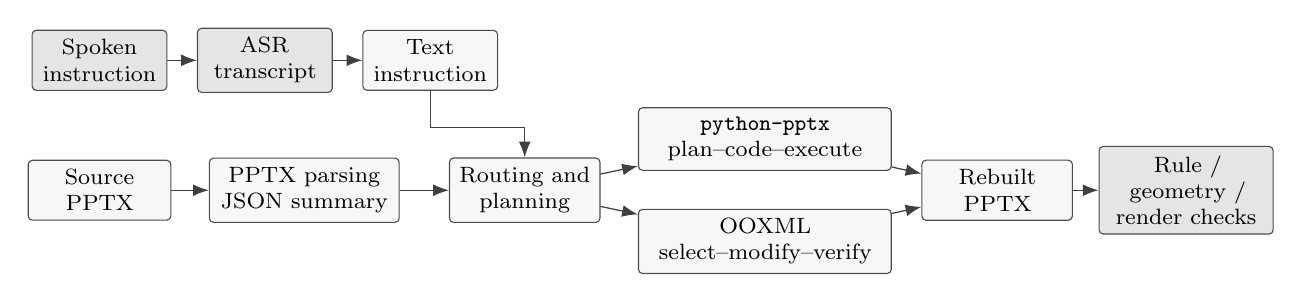
\begin{tikzpicture}[
  x=1cm,y=1cm,
  box/.style={draw=black!70, rounded corners=1.5pt, align=center, minimum height=7.5mm, inner xsep=3pt, fill=black!3, font=\footnotesize},
  added/.style={box, fill=black!10},
  arrow/.style={-{Latex[length=2mm]}, line width=0.45pt, draw=black!75}
]
\node[added, text width=15mm] (audio) at (0.8,1.65) {Spoken instruction};
\node[added, text width=15mm] (asr) at (2.9,1.65) {ASR transcript};
\node[box, text width=15mm] (text) at (5.0,1.65) {Text instruction};
\node[box, text width=16mm] (pptx) at (0.8,0) {Source PPTX};
\node[box, text width=22mm] (parse) at (3.4,0) {PPTX parsing\\JSON summary};
\node[box, text width=17mm] (route) at (6.2,0) {Routing and planning};
\node[box, text width=30mm] (python) at (9.25,0.65) {\texttt{python-pptx}\\plan--code--execute};
\node[box, text width=30mm] (xml) at (9.25,-0.65) {OOXML\\select--modify--verify};
\node[box, text width=17mm] (out) at (12.2,0) {Rebuilt PPTX};
\node[added, text width=20mm] (verify) at (14.6,0) {Rule / geometry /\\render checks};
\draw[arrow] (audio) -- (asr);
\draw[arrow] (asr) -- (text);
\draw[arrow] (pptx) -- (parse);
\draw[arrow] (text) -- (5.0,0.8) -| (route);
\draw[arrow] (parse) -- (route);
\draw[arrow] (route) -- (python);
\draw[arrow] (route) -- (xml);
\draw[arrow] (python) -- (out);
\draw[arrow] (xml) -- (out);
\draw[arrow] (out) -- (verify);
\end{tikzpicture}
\caption{PPTPilot's core editing workflow and the speech-input and verification stages added in this project. Shaded nodes denote project extensions.}
\end{figure}

At execution time, the system first parses a PPTX file into a JSON summary containing slides, objects, text, coordinates, and style information. A routing model then selects the execution path. Standard formatting and batch object operations are performed through \texttt{python-pptx}, whereas complex structural or low-level style changes are implemented by directly modifying and repackaging OOXML. Beyond the original framework, this project added ASR, execution tracing, and independent output verification.

\subsection{Data Source and Experimental Subset}

The tasks were drawn from TSBench, introduced in the \textit{Talk to Your Slides} paper. TSBench Original contains 379 slide-editing instructions. For each instruction, the data team prepared four spoken formulations and rendered each formulation under four acoustic conditions---clean, bandlimit, noise, and reverb---producing $379\times4\times4=6{,}064$ WAV files. The resulting corpus was delivered as \texttt{SSFT260706\_1} and \texttt{SSFT260706\_2}.

\begin{figure}[H]
\centering
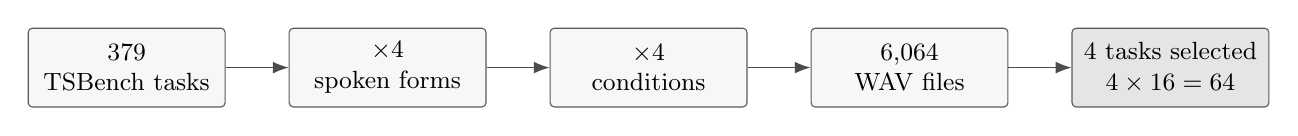
\begin{tikzpicture}[
  box/.style={draw=black!65, rounded corners=1.5pt, align=center, minimum height=10mm, minimum width=25mm, fill=black!3, font=\small},
  arrow/.style={-{Latex[length=2mm]}, line width=0.45pt, draw=black!70},
  node distance=8mm
]
\node[box] (tasks) {379\\TSBench tasks};
\node[box, right=of tasks] (spoken) {$\times 4$\\spoken forms};
\node[box, right=of spoken] (acoustic) {$\times 4$\\conditions};
\node[box, right=of acoustic] (all) {6,064\\WAV files};
\node[box, right=of all, fill=black!10] (subset) {4 tasks selected\\$4\times16=64$};
\draw[arrow] (tasks) -- (spoken);
\draw[arrow] (spoken) -- (acoustic);
\draw[arrow] (acoustic) -- (all);
\draw[arrow] (all) -- (subset);
\end{tikzpicture}
\caption{Corpus expansion procedure and the experimental scope of this report.}
\end{figure}

Four representative editing tasks were selected from the full audio collection: id5 (text correction), id20 (title font size), id31 (horizontal image centering), and id47 (slide-number insertion in the lower-right corner). Each task covered four spoken variants and four acoustic conditions, yielding 64 audio inputs. The corresponding PPTX files and editing instructions originated from TSBench, while the audio variants were produced by the data team.

\section{Development Process and Stage Outputs}

\begin{table}[H]
\centering
\caption{Project stages and completed work}
\small
\begin{tabularx}{\textwidth}{L{2.5cm} Y Y}
\toprule
Stage & Work completed & Principal output (name and role) \\
\midrule
Source-code adaptation & Fixed absolute paths, model configuration, API calls, and output-directory handling & \texttt{PPTArena-main}: locally repaired baseline \\
GUI reproduction & Reproduced the paper's interaction workflow; added model selection, error handling, and result persistence & \texttt{PPTArena\_GUI}: reproduced GUI version \\
CLI refactoring & Removed Flask, front-end, session, and deployment modules; added single-case and batch entry points & \texttt{PPTArena\_CLI}: CLI batch-processing version \\
Speech extension & Integrated faster-whisper and Qwen3-ASR, preserved transcripts, and connected transcription to editing & \texttt{PPTAgent}: first-stage speech-enabled version \\
Final experiments & Replaced the planning and editing models with DeepSeek variants; ran the speech subset and added output verification & \texttt{Agent}: final experimental version \\
\bottomrule
\end{tabularx}
\end{table}

The core codebase decreased from approximately 6,298 lines in the GUI stage to 3,276 lines in the CLI stage and 2,468 lines in the final agent. This reduction primarily resulted from removing the Web interaction, session, and deployment layers. Core capabilities---including PowerPoint parsing, planning, and the dual OOXML/\texttt{python-pptx} editing paths---were retained; the lower line count was not achieved by removing editing functionality.

\subsection{Stage-by-Stage Evolution}

The successive versions formed a progressive development sequence. The initial GUI reproduction made it possible to observe PPTPilot's routing, editing, and preview processes and to confirm that the core framework operated locally. As the number of test cases increased, Web interaction, session state, and manual operations became constraints on batch experimentation. The system was therefore refactored into a CLI with explicit control over inputs, models, editing passes, logs, and output directories.

On top of the CLI, two ASR systems were added as the speech-input layer. Transcripts, agent logs, and edited PPTX files were stored separately, enabling ASR information loss to be distinguished from agent execution errors. Rule-based, geometric, and rendered-slide verification were then introduced, advancing the system from simple executability to batch comparison and failure localization.

\subsection{Final System}

The final system places ASR before PPTPilot's text-instruction interface and adds independent rule-based, geometric, and rendered-slide verification at the output stage. Complex structural modifications use OOXML, while simpler or repetitive operations use \texttt{python-pptx}. In the final configuration, DeepSeek V4 Flash performs planning, and DeepSeek V4 Pro generates editing code or XML modifications.

The unified \texttt{run.py} entry point supports individual audio files, directory-level batch processing, ASR selection, configurable editing passes, and reuse of existing transcripts. Transcripts, edited PPTX files, and logs are stored separately to support reproduction and error localization.

\section{Experimental Design}

\subsection{Data}

The complete audio collection contains 6,064 mono WAV files sampled at 24 kHz, with a total duration of approximately 13.87 hours. It combines 379 instructions, four spoken variants, and four acoustic conditions.

The final experiment selected four PowerPoint editing tasks from the data organized by TSBench task identifier. Each task contained four spoken variants under four acoustic conditions, for 16 recordings per task and 64 recordings overall. The same audio files were processed by two ASR systems:

\begin{itemize}
  \item ASR-2: faster-whisper large-v3-turbo;
  \item ASR-6: Qwen3-ASR-1.7B.
\end{itemize}

\subsection{Tasks}

\begin{table}[H]
\centering
\caption{The four tasks used in the final experiment}
\small
\begin{tabularx}{\textwidth}{C{1.2cm} L{5.2cm} Y L{3.1cm}}
\toprule
Task & Target edit & Principal capability & Verification method \\
\midrule
id5 & Correct spelling, grammar, and typographic errors & Text modification & Text rules \\
id20 & Set all titles to 32 pt & Numeric slots, object identification, batch formatting & Title-size rules \\
id31 & Arrange images horizontally and center the group & Multi-object spatial layout & Geometry and rendering checks \\
id47 & Add slide numbers in the lower-right corner & Structural insertion and positional constraints & Text and coordinate rules \\
\bottomrule
\end{tabularx}
\end{table}

These four tasks form a progression from simple text correction to precise formatting, structural insertion, and spatial layout. They constitute the experimental subset used to validate the current system pipeline and do not represent the full task coverage of TSBench.

\subsection{Evaluation Criteria}

The outputs were evaluated at four levels:

\begin{enumerate}
  \item \textbf{Readable output:} whether an openable PPTX file was generated;
  \item \textbf{Edit signal:} whether the output differed from the input;
  \item \textbf{Rule correctness:} whether the target text, font-size, or slide-number constraints were satisfied;
  \item \textbf{Geometric correctness:} whether objects overlapped, exceeded slide boundaries, or were incorrectly positioned.
\end{enumerate}

Accordingly, a readable output indicates only that file generation completed. An editing task was counted as successful only when its target text, formatting, or geometric constraints were also satisfied.

\section{Experimental Results}

\subsection{Overall First-Pass Results}

\begin{table}[H]
\centering
\caption{First-pass end-to-end results for the two ASR systems}
\small
\begin{tabularx}{\textwidth}{Y C{3.1cm} C{3.1cm} C{2.2cm}}
\toprule
Metric & ASR-2 & ASR-6 & Difference / pp \\
\midrule
Readable final PPTX generated & 61/64 (95.31\%) & 63/64 (98.44\%) & +3.13 \\
Output with an edit signal & 52/64 (81.25\%) & 60/64 (93.75\%) & +12.50 \\
Correct under rule-based verification (id5, id20, id47) & 32/48 (66.67\%) & 38/48 (79.17\%) & +12.50 \\
Correct under geometric and visual verification (id31) & 10/16 (62.50\%) & 10/16 (62.50\%) & 0.00 \\
Correct under task-specific verification & 42/64 (65.63\%) & 48/64 (75.00\%) & +9.37 \\
\bottomrule
\end{tabularx}
\end{table}

The 48 rule-evaluated cases comprise id5, id20, and id47, for which deterministic checks were available. The 16 first-pass id31 outputs were evaluated separately using geometric measurements and rendered-slide inspection. ASR-6 improved both output rate and accuracy on the three rule-based tasks, but overall task-specific accuracy remained 75.00\%. Thus, a readable PPTX and an editing log establish only that the pipeline ran; the agent may still make substantive errors in object identification, planning, or execution.

\begin{figure}[H]
\centering
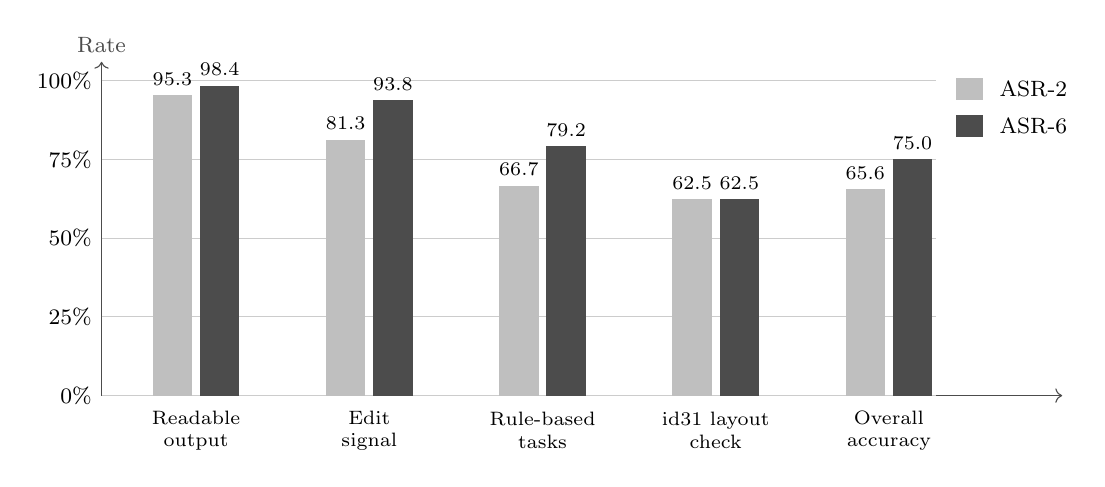
\begin{tikzpicture}[x=1cm,y=0.040cm,font=\footnotesize]
\draw[->,black!70] (0,0) -- (0,106) node[above] {Rate};
\draw[->,black!70] (0,0) -- (12.2,0);
\foreach \y in {0,25,50,75,100} {
  \draw[black!20] (0,\y) -- (10.6,\y);
  \node[left] at (0,\y) {\y\%};
}
\fill[black!25] (0.65,0) rectangle (1.15,95.31);
\fill[black!70] (1.25,0) rectangle (1.75,98.44);
\node[above,font=\scriptsize] at (0.90,95.31) {95.3};
\node[above,font=\scriptsize] at (1.50,98.44) {98.4};
\node[align=center,font=\scriptsize] at (1.20,-11) {Readable\\output};

\fill[black!25] (2.85,0) rectangle (3.35,81.25);
\fill[black!70] (3.45,0) rectangle (3.95,93.75);
\node[above,font=\scriptsize] at (3.10,81.25) {81.3};
\node[above,font=\scriptsize] at (3.70,93.75) {93.8};
\node[align=center,font=\scriptsize] at (3.40,-11) {Edit\\signal};

\fill[black!25] (5.05,0) rectangle (5.55,66.67);
\fill[black!70] (5.65,0) rectangle (6.15,79.17);
\node[above,font=\scriptsize] at (5.30,66.67) {66.7};
\node[above,font=\scriptsize] at (5.90,79.17) {79.2};
\node[align=center,font=\scriptsize] at (5.60,-11) {Rule-based\\tasks};

\fill[black!25] (7.25,0) rectangle (7.75,62.50);
\fill[black!70] (7.85,0) rectangle (8.35,62.50);
\node[above,font=\scriptsize] at (7.50,62.50) {62.5};
\node[above,font=\scriptsize] at (8.10,62.50) {62.5};
\node[align=center,font=\scriptsize] at (7.80,-11) {id31 layout\\check};

\fill[black!25] (9.45,0) rectangle (9.95,65.63);
\fill[black!70] (10.05,0) rectangle (10.55,75.00);
\node[above,font=\scriptsize] at (9.70,65.63) {65.6};
\node[above,font=\scriptsize] at (10.30,75.00) {75.0};
\node[align=center,font=\scriptsize] at (10.00,-11) {Overall\\accuracy};

\fill[black!25] (10.85,94) rectangle (11.20,101);
\node[right] at (11.28,97.5) {ASR-2};
\fill[black!70] (10.85,82) rectangle (11.20,89);
\node[right] at (11.28,85.5) {ASR-6};
\end{tikzpicture}
\caption{First-pass end-to-end metrics for the two ASR systems. Qwen3-ASR improved readable output, edit signal, rule-based task performance, and overall accuracy, while id31 remained unchanged.}
\end{figure}

\subsection{Task-Level Results}

\begin{table}[H]
\centering
\caption{First-pass verification results for the four tasks}
\small
\begin{tabularx}{\textwidth}{L{4.4cm} C{2.6cm} C{2.6cm} Y}
\toprule
Task & ASR-2 & ASR-6 & Interpretation \\
\midrule
id5 spelling and grammar & 16/16 & 16/16 & Relatively stable \\
id20 title size (32 pt) & 2/16 & 7/16 & Principal bottleneck \\
id31 horizontal image centering & 10/16 & 10/16 & Layout planning remains unstable \\
id47 lower-right slide numbers & 14/16 & 15/16 & Generally reliable \\
Total & 42/64 (65.63\%) & 48/64 (75.00\%) & ASR-6 higher by 9.37 pp \\
\bottomrule
\end{tabularx}
\end{table}

\begin{figure}[H]
\centering
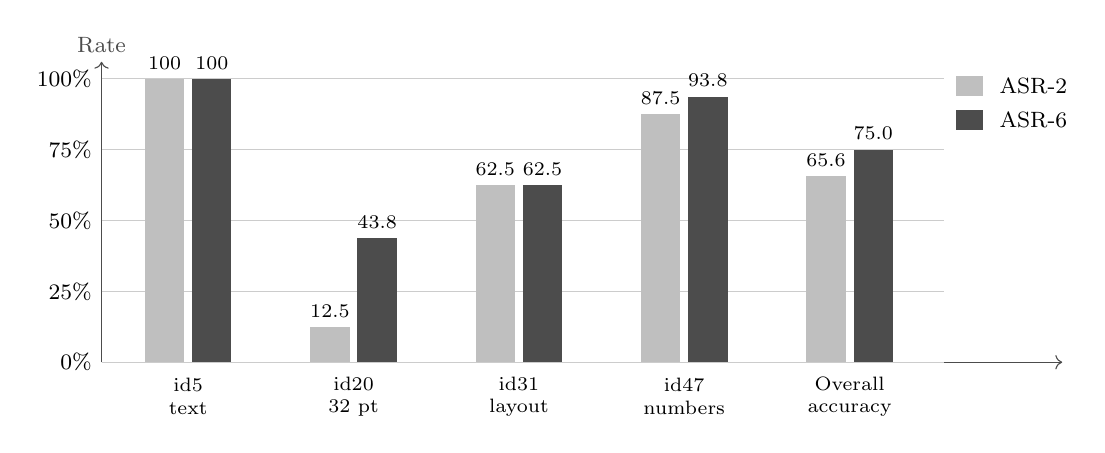
\begin{tikzpicture}[x=1cm,y=0.036cm,font=\footnotesize]
\draw[->,black!70] (0,0) -- (0,106) node[above] {Rate};
\draw[->,black!70] (0,0) -- (12.2,0);
\foreach \y in {0,25,50,75,100} {
  \draw[black!20] (0,\y) -- (10.7,\y);
  \node[left] at (0,\y) {\y\%};
}
\fill[black!25] (0.55,0) rectangle (1.05,100.00);
\fill[black!70] (1.15,0) rectangle (1.65,100.00);
\node[above,font=\scriptsize] at (0.80,100.00) {100};
\node[above,font=\scriptsize] at (1.40,100.00) {100};
\node[align=center,font=\scriptsize] at (1.10,-12) {id5\\text};

\fill[black!25] (2.65,0) rectangle (3.15,12.50);
\fill[black!70] (3.25,0) rectangle (3.75,43.75);
\node[above,font=\scriptsize] at (2.90,12.50) {12.5};
\node[above,font=\scriptsize] at (3.50,43.75) {43.8};
\node[align=center,font=\scriptsize] at (3.20,-12) {id20\\32 pt};

\fill[black!25] (4.75,0) rectangle (5.25,62.50);
\fill[black!70] (5.35,0) rectangle (5.85,62.50);
\node[above,font=\scriptsize] at (5.00,62.50) {62.5};
\node[above,font=\scriptsize] at (5.60,62.50) {62.5};
\node[align=center,font=\scriptsize] at (5.30,-12) {id31\\layout};

\fill[black!25] (6.85,0) rectangle (7.35,87.50);
\fill[black!70] (7.45,0) rectangle (7.95,93.75);
\node[above,font=\scriptsize] at (7.10,87.50) {87.5};
\node[above,font=\scriptsize] at (7.70,93.75) {93.8};
\node[align=center,font=\scriptsize] at (7.40,-12) {id47\\numbers};

\fill[black!25] (8.95,0) rectangle (9.45,65.63);
\fill[black!70] (9.55,0) rectangle (10.05,75.00);
\node[above,font=\scriptsize] at (9.20,65.63) {65.6};
\node[above,font=\scriptsize] at (9.80,75.00) {75.0};
\node[align=center,font=\scriptsize] at (9.50,-12) {Overall\\accuracy};

\fill[black!25] (10.85,94) rectangle (11.20,101);
\node[right] at (11.28,97.5) {ASR-2};
\fill[black!70] (10.85,82) rectangle (11.20,89);
\node[right] at (11.28,85.5) {ASR-6};
\end{tikzpicture}
\caption{First-pass accuracy for the four tasks. Id31 was evaluated geometrically and visually; the remaining tasks used deterministic rules.}
\end{figure}

Id5 achieved 100\% under both ASR systems, indicating that simple text correction was already relatively stable. Id20 performed worst, demonstrating persistent difficulty with exact numeric values, title-object identification, and formatting changes. Id31 was assessed using geometry and rendered slides, whereas the other three tasks used deterministic rules. The total therefore reports first-pass correctness under the task-appropriate verification method.

\subsection{Targeted Second-Pass Experiment}

After the first pass, two poorly performing task groups were selected for a second editing pass: the 16 id20 cases under ASR-2 and the 16 id31 cases under each of ASR-2 and ASR-6, for 48 matched cases in total. The reruns reused the same transcripts; the second pass replanned and executed against the current PowerPoint state. Here, ``targeted'' means that difficult task groups were selected for additional runs, not that a verifier triggered retries only for first-pass failures.

\begin{table}[H]
\centering
\caption{Targeted second pass: final states of matched cases after one and two editing passes}
\small
\begin{tabularx}{\textwidth}{Y C{2.1cm} C{2.1cm} C{2.0cm} C{2.0cm} C{1.5cm}}
\toprule
Task / ASR & First-pass readable & Second-pass readable & First-pass correct & Second-pass correct & $\Delta$ / pp \\
\midrule
id20 / ASR-2 & 16/16 & 16/16 & 2/16 (12.50\%) & 3/16 (18.75\%) & +6.25 \\
id31 / ASR-2 & 14/16 & 15/16 & 10/16 (62.50\%) & 8/16 (50.00\%) & -12.50 \\
id31 / ASR-6 & 15/16 & 13/16 & 10/16 (62.50\%) & 9/16 (56.25\%) & -6.25 \\
\midrule
Total & 45/48 (93.75\%) & 44/48 (91.67\%) & 22/48 (45.83\%) & 20/48 (41.67\%) & -4.17 \\
\bottomrule
\end{tabularx}
\end{table}

\begin{figure}[H]
\centering
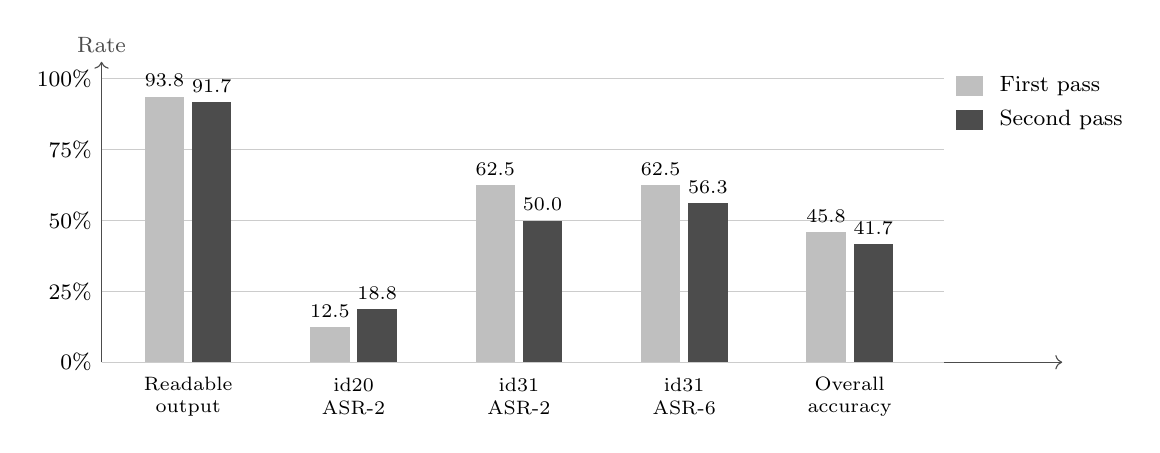
\begin{tikzpicture}[x=1cm,y=0.036cm,font=\footnotesize]
\draw[->,black!70] (0,0) -- (0,106) node[above] {Rate};
\draw[->,black!70] (0,0) -- (12.2,0);
\foreach \y in {0,25,50,75,100} {
  \draw[black!20] (0,\y) -- (10.7,\y);
  \node[left] at (0,\y) {\y\%};
}
\fill[black!25] (0.55,0) rectangle (1.05,93.75);
\fill[black!70] (1.15,0) rectangle (1.65,91.67);
\node[above,font=\scriptsize] at (0.80,93.75) {93.8};
\node[above,font=\scriptsize] at (1.40,91.67) {91.7};
\node[align=center,font=\scriptsize] at (1.10,-12) {Readable\\output};

\fill[black!25] (2.65,0) rectangle (3.15,12.50);
\fill[black!70] (3.25,0) rectangle (3.75,18.75);
\node[above,font=\scriptsize] at (2.90,12.50) {12.5};
\node[above,font=\scriptsize] at (3.50,18.75) {18.8};
\node[align=center,font=\scriptsize] at (3.20,-12) {id20\\ASR-2};

\fill[black!25] (4.75,0) rectangle (5.25,62.50);
\fill[black!70] (5.35,0) rectangle (5.85,50.00);
\node[above,font=\scriptsize] at (5.00,62.50) {62.5};
\node[above,font=\scriptsize] at (5.60,50.00) {50.0};
\node[align=center,font=\scriptsize] at (5.30,-12) {id31\\ASR-2};

\fill[black!25] (6.85,0) rectangle (7.35,62.50);
\fill[black!70] (7.45,0) rectangle (7.95,56.25);
\node[above,font=\scriptsize] at (7.10,62.50) {62.5};
\node[above,font=\scriptsize] at (7.70,56.25) {56.3};
\node[align=center,font=\scriptsize] at (7.40,-12) {id31\\ASR-6};

\fill[black!25] (8.95,0) rectangle (9.45,45.83);
\fill[black!70] (9.55,0) rectangle (10.05,41.67);
\node[above,font=\scriptsize] at (9.20,45.83) {45.8};
\node[above,font=\scriptsize] at (9.80,41.67) {41.7};
\node[align=center,font=\scriptsize] at (9.50,-12) {Overall\\accuracy};

\fill[black!25] (10.85,94) rectangle (11.20,101);
\node[right] at (11.28,97.5) {First pass};
\fill[black!70] (10.85,82) rectangle (11.20,89);
\node[right] at (11.28,85.5) {Second pass};
\end{tikzpicture}
\caption{Final results after one and two passes in the targeted reruns. Accuracy was determined by the id20 rule-based verifier and the id31 geometric/rendered-slide verifier.}
\end{figure}

Case-level comparison reveals changes concealed by aggregate counts. For id20, one case remained correct, one changed from correct to incorrect, and two changed from incorrect to correct, yielding a net gain of one. Among the 32 id31 cases, 10 of the 20 first-pass successes became incorrect after the second pass, while only 7 of the 12 first-pass failures were repaired, producing a net loss of three. Overall correctness therefore declined from 22/48 to 20/48 not because the second pass was wholly ineffective, but because it damaged some previously correct results while repairing a subset of failures.

The additional pass also increased computational and execution cost. Automatic retry events recorded in the corresponding logs rose from 3 in the first-pass runs to 15 in the two-pass runs, while readable outputs decreased from 45/48 to 44/48. Full replanning and re-execution therefore introduced new code-generation and layout risks. A preferable strategy would preserve the first-pass output and use rule-based or geometric verifiers to trigger targeted retries only for failed cases.

\subsection{Critical Slot: 32 pt}

Post hoc inspection of the id20 transcripts yielded the following results:

\begin{table}[H]
\centering
\caption{Preservation of the id20 critical slot and downstream correctness}
\small
\begin{tabularx}{0.78\textwidth}{Y C{3.2cm} C{3.2cm}}
\toprule
Metric & ASR-2 & ASR-6 \\
\midrule
Transcript fully preserved ``32 pt'' & 3/16 & 7/16 \\
Correct under downstream rules & 2/16 & 7/16 \\
\bottomrule
\end{tabularx}
\end{table}

ASR-6's improvement arose primarily from better preservation of the critical value and unit. However, one ASR-2 transcript retained ``32 pt'' while the downstream edit still failed. Accurate ASR is therefore one necessary condition for end-to-end success, but it is not sufficient.

\subsection{Image-Centering Task: Geometric and Visual Inspection}

Id31 requires the three existing images to be arranged horizontally and centered as a group. An edit signal alone cannot determine whether this layout is correct; consequently, the task was evaluated using both PPTX object geometry and rendered-slide inspection. The 64 final states produced by two ASR systems, two editing passes, and 16 spoken/acoustic combinations were classified as pass, image overlap, positional error, or missing output.

\begin{table}[H]
\centering
\caption{Verification results for final id31 states}
\small
\begin{tabularx}{\textwidth}{Y C{1.4cm} C{1.7cm} C{1.5cm} C{1.5cm} C{1.7cm} C{1.8cm}}
\toprule
ASR & Pass & Correct & Overlap & Offset & No output & Success rate \\
\midrule
ASR-2 & First & 10/16 & 3 & 1 & 2 & 62.5\% \\
ASR-2 & Second & 8/16 & 7 & 0 & 1 & 50.0\% \\
ASR-6 & First & 10/16 & 3 & 2 & 1 & 62.5\% \\
ASR-6 & Second & 9/16 & 4 & 0 & 3 & 56.3\% \\
\midrule
Total & --- & 37/64 & 17 & 3 & 7 & 57.8\% \\
\bottomrule
\end{tabularx}
\end{table}

All 57 generated PPTX files retained the three original images. The failures did not result from deleted media; rather, the agent often aligned multiple images to the same page center. Overlap occurred in 17 cases: two images overlapped in 14 cases, and all three overlapped in 3. A further 3 cases were misplaced, and 7 produced no output.

\begin{figure}[H]
\centering
\begin{minipage}[t]{0.485\textwidth}
  \centering
  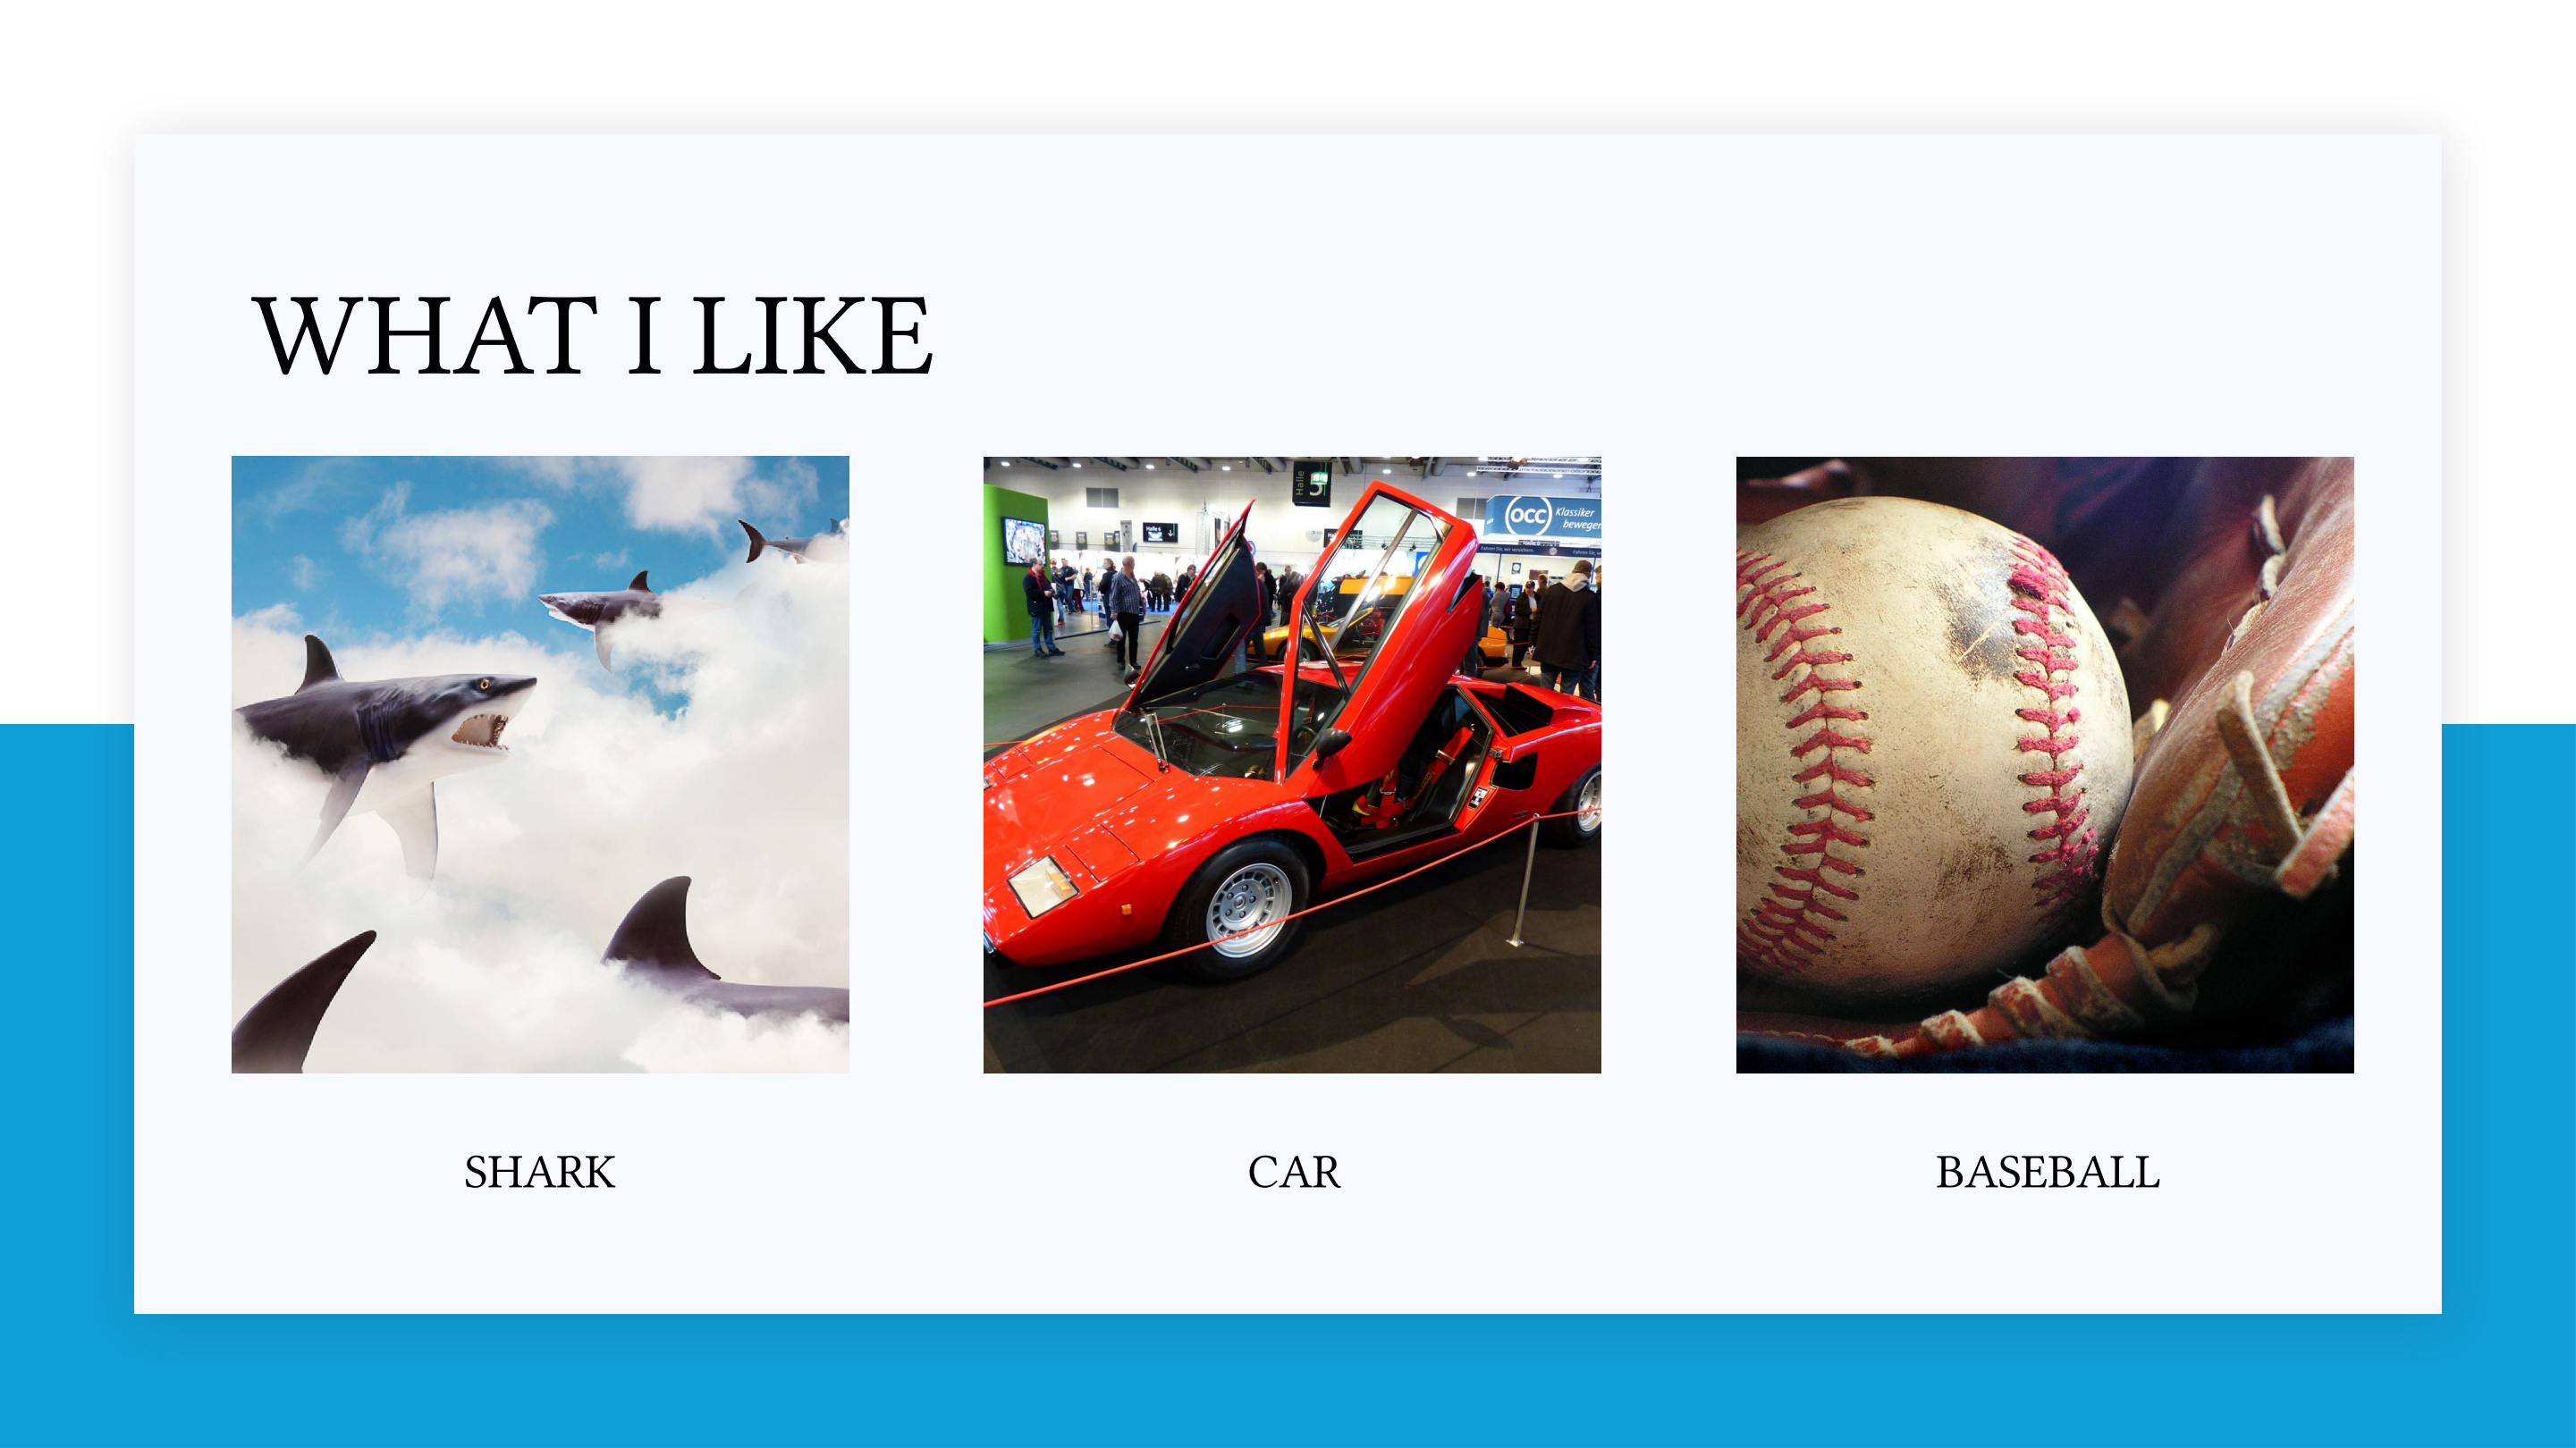
\includegraphics[width=\linewidth]{id31_layout_pass.png}
  {\small (a) Pass: three images distributed at equal spacing}
\end{minipage}\hfill
\begin{minipage}[t]{0.485\textwidth}
  \centering
  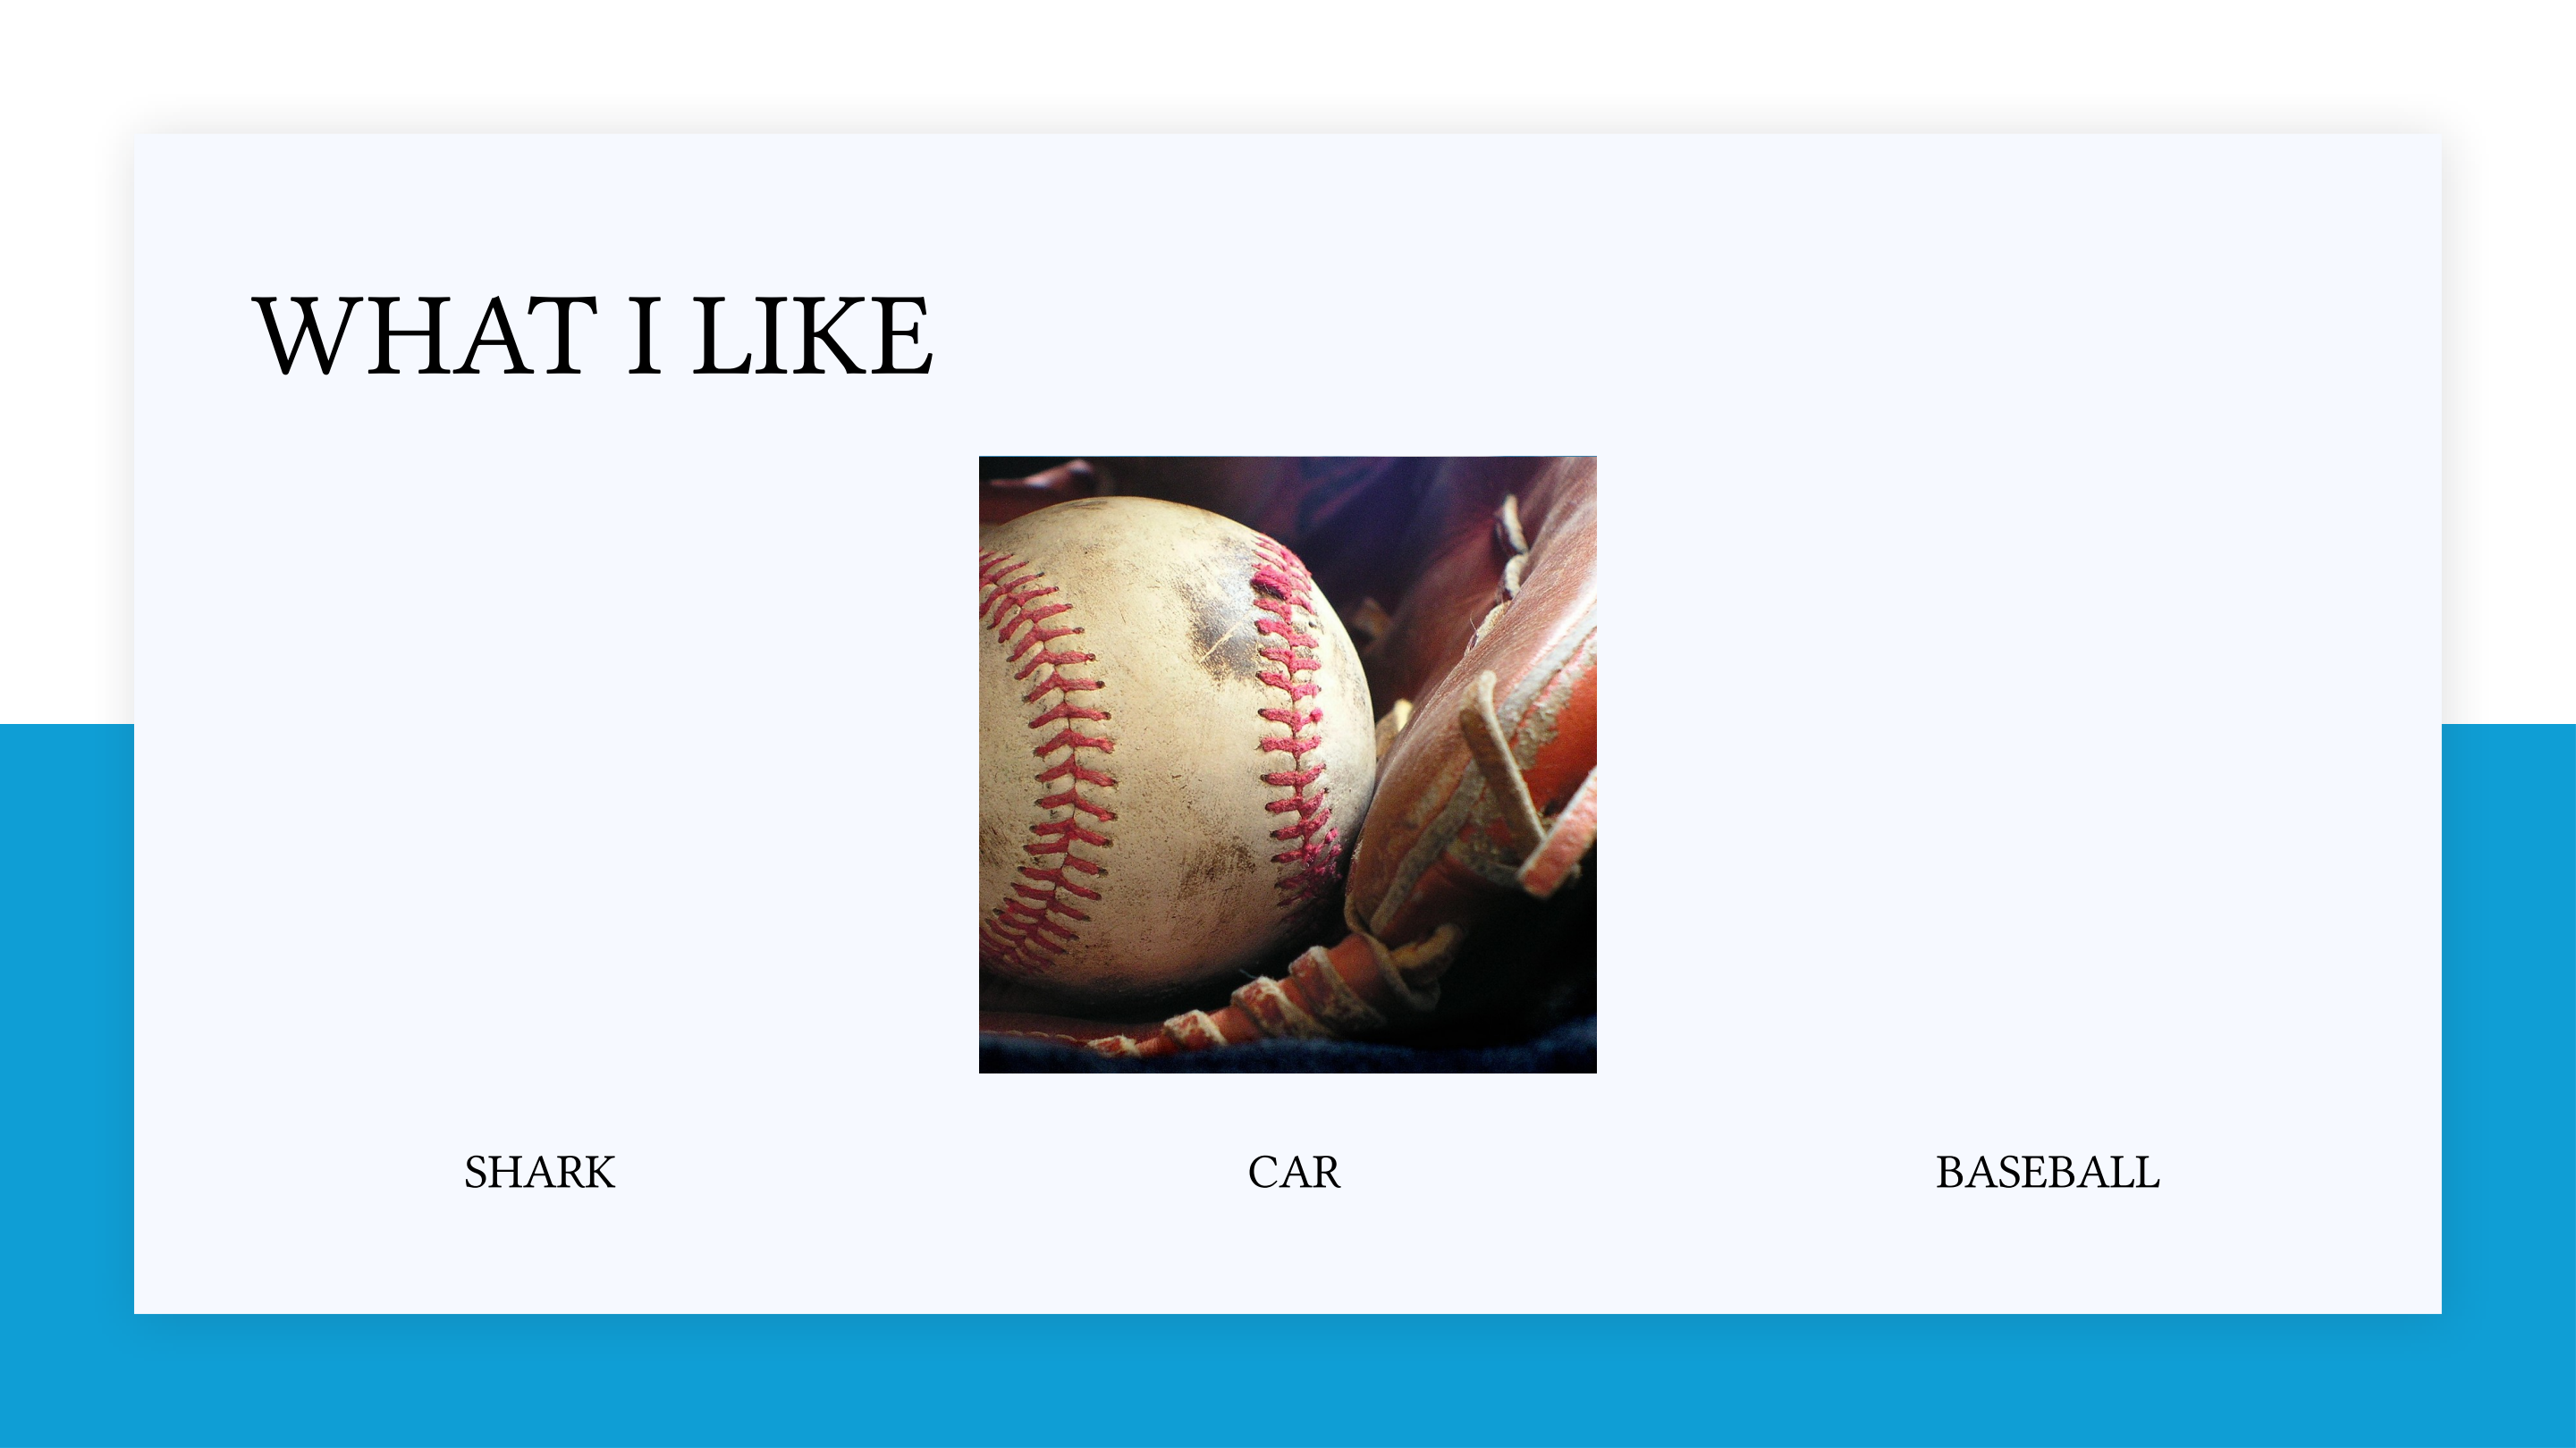
\includegraphics[width=\linewidth]{id31_layout_overlap.png}
  {\small (b) Failure: all three images overlap at the center}
\end{minipage}
\caption{Actual id31 outputs. Left: a passing result. Right: the three original images overlap at the slide center, leaving only the top layer visible.}
\end{figure}

ASR-2 and ASR-6 passed 18/32 and 19/32 cases, respectively, a difference of only 3.1 percentage points. By editing pass, the corresponding totals were 20/32 after the first pass and 17/32 after the second, a decline of 9.4 percentage points. The four acoustic conditions yielded 9/16, 12/16, 7/16, and 9/16 passes, with no stable pattern. The principal bottleneck therefore lies in the agent's spatial reasoning and execution, and targeted retries should be triggered by geometric verification.

\section{Failures, Challenges, and Improvements}

\subsection{Localization of Major Failures}

\begin{table}[H]
\centering
\caption{Major failure stages and supporting evidence}
\small
\begin{tabularx}{\textwidth}{L{2.7cm} L{5.4cm} Y}
\toprule
Failure stage & Experimental evidence & Principal mechanism \\
\midrule
Loss of critical ASR information & For id20, complete preservation of ``32 pt'' increased from 3/16 to 7/16, while downstream correctness increased from 2/16 to 7/16 & Errors in numeric values or units directly alter editing parameters \\
Agent object and layout planning & All 57 existing id31 PPTX files retained three images, yet 17 exhibited overlap and 3 exhibited misplacement & ``Center the arrangement horizontally'' was interpreted as centering each image independently, without a global layout constraint \\
Generated code and API calls & In the 64 first-pass runs, generated-script errors triggered retries in 6 cases & Incorrect access to \texttt{runs[0]} in empty paragraphs and misuse of color APIs, media enumeration, private placeholder attributes, or slide-size properties \\
Loop control and output verification & Id31 correctness declined from 20/32 after one pass to 17/32 after two passes, while overlap increased & Full replanning in the second pass can overwrite correct first-pass results; the system lacks failure-triggered execution, rollback, and state comparison \\
\bottomrule
\end{tabularx}
\end{table}

These failures cannot be attributed uniformly to ASR. In id20, for example, one ASR-2 transcript preserved ``32 pt'' but the downstream edit still failed, showing that the agent may select the wrong object or generate faulty code even when transcription is adequate. Conversely, id31 achieved 10/16 first-pass successes under both ASR systems, and their two-pass totals differed by only 3.1 percentage points. The principal bottleneck for this task therefore lies in object localization and spatial planning.

Stronger planning or code-generation models may reduce syntax errors, API hallucinations, and some object-selection errors, but model capability is only one component. If the system continues to rely on unconstrained generation of low-level API code without object inventories, type constraints, output verification, or rollback, structural errors such as overlap, misplacement, and corruption of existing formatting may persist. Future work should compare agent models while holding the ASR system, tasks, and verifiers fixed, thereby separating the contribution of model capability from that of tool constraints.

\subsection{Engineering Challenges and Current Mitigations}

\begin{table}[H]
\centering
\caption{Engineering challenges, current mitigations, and unresolved issues}
\small
\begin{tabularx}{\textwidth}{L{3.0cm} Y Y}
\toprule
Challenge & Mitigation implemented in this project & Remaining limitation \\
\midrule
Dependence on the authors' environment & Replaced absolute paths and unified input, output, and model configuration & Complete environment locking and one-command deployment remain unavailable \\
GUI unsuitable for batch execution & Refactored the CLI and added entry points for single tasks, directory batches, and transcript reuse & Large-scale checkpoint recovery and configuration manifests require further development \\
Model cost and availability & Adopted affordable DeepSeek models for planning and editing & No systematic capability--cost--latency curve has yet been established \\
Entangled ASR and agent errors & Preserved transcripts, logs, and outputs, and inspected critical slots & Comprehensive slot-level metrics and a structured intent layer remain absent \\
Inconsistent evaluation criteria & Defined rules for text, font size, and slide numbers, and added geometry/rendering checks for layout & Unified verifiers covering more tasks and systematic human auditing are still needed \\
\bottomrule
\end{tabularx}
\end{table}

\subsection{Directions for Further Improvement}

\begin{enumerate}
  \item Introduce a structured intent layer between ASR and the agent that explicitly records actions, target objects, attributes, values, units, and coreference relations, and validates critical slots before execution;
  \item Replace unconstrained low-level API generation with typed editing tools and explicit object inventories that restrict callable functions, parameter ranges, and object scope;
  \item Establish a planning--execution--verification loop in which rules, geometric differences, and rendered outputs trigger targeted retries, while correct first-pass results and rollback checkpoints are preserved;
  \item Extend evaluation to additional TSBench tasks, ASR systems, and editing agents; include a clean-text upper bound, unify failure categories, and report confidence intervals and significance tests.
\end{enumerate}

\section{Research Motivation and Stage-Level Findings}

\subsection{Original Motivation and Scope of This Stage}

The project originally examined how large language models could interpret spoken instructions and execute slide edits. Hesitations, pauses, self-corrections, and informal phrasing, together with acoustic variations such as band limitation, noise, and reverberation, may cause actions, target objects, attributes, or values to be lost during transcription. The original research design therefore extended beyond plain speech-to-text conversion: it also envisioned structured representations of editing intent and comparison of downstream behavior between speech-based input and transcript-only input.

This report completes a transcript-mediated system validation within that broader agenda: two ASR systems process the same speech inputs, PPTPilot executes the resulting instructions, and transcripts, logs, PPTX files, and verification results are retained. The current data are insufficient to estimate a stable independent effect for any single acoustic condition, but they do distinguish two failure classes: loss of critical information during transcription and agent execution failure despite an adequate transcript.

\subsection{Findings Supported at This Stage}

\begin{itemize}
  \item Transcription quality affects editing performance, but its impact is concentrated in task-critical slots. When Qwen3-ASR preserved ``32 pt'' more reliably, id20 correctness increased from 2/16 to 7/16;
  \item A high readable-output rate does not imply a high task-completion rate. ASR-6 produced readable first-pass outputs in 98.44\% of cases, but overall task-specific verification accuracy was 75.00\%;
  \item Correct transcription is not sufficient for task success. Even when critical information is preserved, the agent can fail through object selection, spatial planning, or code execution;
  \item Rendered-slide verification is indispensable. Failed id31 PPTX files still contained all three images; complete occlusion could be detected only by examining object geometry and slide renderings;
  \item A fixed increase in editing passes does not guarantee improvement. Verifier-triggered targeted retries are more appropriate than unconditional repetition.
\end{itemize}

\subsection{Limitations of the Conclusions}

The current experiment covers only four task types, two ASR systems, and one PowerPoint editing agent. It does not include a clean-text upper bound, structured intent representations, speech-native models, or complete statistical testing. The results therefore do not represent the full Speech2SlideEdit/TSBench benchmark, do not establish a stable monotonic effect for any acoustic condition, and do not justify claims of statistically significant model superiority. Their value lies in the reproducible system pipeline, traceable failure evidence, and evaluation framework established for subsequent full-scale experiments.

\section{Conclusion}

Starting from PPTPilot as introduced in the PPTArena paper, this project completed local adaptation, GUI reproduction, CLI refactoring, dual-ASR integration, and speech-driven editing experiments. The final system preserves audio transcripts, agent execution traces, edited PPTX files, and rule-based, geometric, and rendered-slide verification results, forming a complete evidence chain from input to failure analysis.

The results exhibit a clear hierarchy. At the pipeline level, the two ASR systems produced 61/64 and 63/64 readable first-pass outputs. At the semantic level, the stronger ASR system increased accuracy on the three rule-based tasks from 66.67\% to 79.17\% by preserving critical values and units. At the execution level, id31 achieved only 10/16 first-pass successes under each ASR system; its combined two-pass success rate was 57.8\%, with second-pass performance lower overall than first-pass performance. ASR improvements can therefore reduce upstream information loss, but agent object understanding, code reliability, and output control remain the principal limitations of the end-to-end system.

Across the 48 matched cases comprising id20 under ASR-2 and id31 under both ASR systems, final correctness declined from 22/48 after one pass to 20/48 after two, while automatic retry events recorded in the logs increased from 3 to 15. The second pass both repaired failures and overwrote correct results; it should therefore not be adopted as a default strategy.

Future work should jointly develop representations of task-critical information, constrained editing tools, geometric and rendered-slide verifiers, and rollback-capable targeted retry mechanisms.

\section*{References}

\begin{enumerate}[label={[\arabic*]},leftmargin=2.5em]
  \item Michael Ofengenden, Yunze Man, Ziqi Pang, Yu-Xiong Wang. \textit{PPTArena: A Benchmark for Agentic PowerPoint Editing}. arXiv:2512.03042v2, 2025.
  \item Kyudan Jung et al. \textit{Talk to Your Slides: High-Efficiency Slide Editing via Language-Driven Structured Data Manipulation}. arXiv:2505.11604v4, 2026.
  \item SURF-2026-0425 project description and internal experimental materials.
  \item Project source code, stage reports, experimental outputs, and audit records, June--July 2026.
\end{enumerate}

\appendix
\section{Index of Principal Outputs}

\begingroup
\footnotesize
\renewcommand{\arraystretch}{1.05}
\setlength{\LTpre}{0.3em}
\setlength{\LTpost}{0pt}
\begin{longtable}{L{2.9cm} L{3.0cm} L{8.6cm}}
\toprule
Output & Role & Description \\
\midrule
\endfirsthead
\toprule
Output & Role & Description \\
\midrule
\endhead
PPTArena-main & Original baseline & Released paper code and starting point for local repairs \\
PPTArena\_GUI & GUI reproduction & Local preview, model selection, error handling, and result persistence \\
PPTArena\_CLI & Batch-processing foundation & Single-case and batch entry points without Web dependencies \\
Early GUI/CLI result comparison & Exploratory experiment & Inputs, outputs, and GUI/CLI records for 10 cases selected from the PPTArena dataset; not a controlled paired comparison \\
PPTAgent & First speech extension & Dual ASR integration, task mapping, and transcript persistence \\
Agent & Final experimental version & Unified entry point, DeepSeek models, four-task outputs, rule/geometric verification, case-level audit, and final report \\
SSFT260706\_1 / \_2 & Audio collection & Four spoken variants under clean, bandlimit, noise, and reverb conditions \\
\bottomrule
\end{longtable}
\endgroup

\end{document}
